\documentclass[]{article}
\usepackage{lmodern}
\usepackage{amssymb,amsmath}
\usepackage{ifxetex,ifluatex}
\usepackage{fixltx2e} % provides \textsubscript
\ifnum 0\ifxetex 1\fi\ifluatex 1\fi=0 % if pdftex
  \usepackage[T1]{fontenc}
  \usepackage[utf8]{inputenc}
\else % if luatex or xelatex
  \ifxetex
    \usepackage{mathspec}
  \else
    \usepackage{fontspec}
  \fi
  \defaultfontfeatures{Ligatures=TeX,Scale=MatchLowercase}
\fi
% use upquote if available, for straight quotes in verbatim environments
\IfFileExists{upquote.sty}{\usepackage{upquote}}{}
% use microtype if available
\IfFileExists{microtype.sty}{%
\usepackage{microtype}
\UseMicrotypeSet[protrusion]{basicmath} % disable protrusion for tt fonts
}{}
\usepackage[margin=1in]{geometry}
\usepackage{hyperref}
\hypersetup{unicode=true,
            pdftitle={Predicting Job Mismatch Rate Through Job Satisfaction - PPOL 670 Group Project},
            pdfauthor={Connor Harrison, Dong Hoon Lee, Haorui Sun},
            pdfborder={0 0 0},
            breaklinks=true}
\urlstyle{same}  % don't use monospace font for urls
\usepackage{graphicx,grffile}
\makeatletter
\def\maxwidth{\ifdim\Gin@nat@width>\linewidth\linewidth\else\Gin@nat@width\fi}
\def\maxheight{\ifdim\Gin@nat@height>\textheight\textheight\else\Gin@nat@height\fi}
\makeatother
% Scale images if necessary, so that they will not overflow the page
% margins by default, and it is still possible to overwrite the defaults
% using explicit options in \includegraphics[width, height, ...]{}
\setkeys{Gin}{width=\maxwidth,height=\maxheight,keepaspectratio}
\IfFileExists{parskip.sty}{%
\usepackage{parskip}
}{% else
\setlength{\parindent}{0pt}
\setlength{\parskip}{6pt plus 2pt minus 1pt}
}
\setlength{\emergencystretch}{3em}  % prevent overfull lines
\providecommand{\tightlist}{%
  \setlength{\itemsep}{0pt}\setlength{\parskip}{0pt}}
\setcounter{secnumdepth}{0}
% Redefines (sub)paragraphs to behave more like sections
\ifx\paragraph\undefined\else
\let\oldparagraph\paragraph
\renewcommand{\paragraph}[1]{\oldparagraph{#1}\mbox{}}
\fi
\ifx\subparagraph\undefined\else
\let\oldsubparagraph\subparagraph
\renewcommand{\subparagraph}[1]{\oldsubparagraph{#1}\mbox{}}
\fi

%%% Use protect on footnotes to avoid problems with footnotes in titles
\let\rmarkdownfootnote\footnote%
\def\footnote{\protect\rmarkdownfootnote}

%%% Change title format to be more compact
\usepackage{titling}

% Create subtitle command for use in maketitle
\newcommand{\subtitle}[1]{
  \posttitle{
    \begin{center}\large#1\end{center}
    }
}

\setlength{\droptitle}{-2em}

  \title{Predicting Job Mismatch Rate Through Job Satisfaction - PPOL 670 Group
Project}
    \pretitle{\vspace{\droptitle}\centering\huge}
  \posttitle{\par}
    \author{Connor Harrison, Dong Hoon Lee, Haorui Sun}
    \preauthor{\centering\large\emph}
  \postauthor{\par}
      \predate{\centering\large\emph}
  \postdate{\par}
    \date{April 28, 2019}


\begin{document}
\maketitle

\section{Method Section}\label{method-section}

The first approach we took in answering our hypothesis is using data
visualizations to look for patterns and relationships between the
dependent variable and independent variable while controlling for
difference in characteristics such as region, race, highest degree
attained, job sector, age, and company size. And because survey data set
contained one variable for overall satisfaction at the job and one for
each aspects of the job, we decided to use all the job satisfaction
variables for the visualization analysis to look for additional insights
about different types of job satisfaction.

The first step to visualization analysis was to recode variables to be
suitable for visualization. The original satisfaction variables had the
following four possible responses: ``very dissatisfied,''
``dissatisfied,'' ``satisfied,'' and ``very satisfied.'' For the
purposes easier presentation and interpretation, we created an indicator
for those who reported as ``satisfied'' or ``very satisfied'' with their
job or aspects of the job. The key independent variable, undergraduate
student loan amount, was also ordinally categorized with the starting
loan amount of \$0 and going up in the increments of \$10,000 up to
\$90,000, at which point was grouped in to more than \$90,000. Because
the values of this variable were not numerical to begin with, we grouped
loan amounts into increments of \$30,000 (e.g.~between \$1 - \$30,000
and \$30,000 - 60,000) with the last value group consisting of those
with more than \$90,000 of loan.

We first looked at the overall distribution of loan amounts by race
groups and region to see if there's any significant differences in terms
of loan borrowing trends. Then we plotted overall job satisfaction level
by loan amount groups in different regions and then by race and
ethnicity groups. Lastly, we plotted the average satisfaction level in
their jobs and in various aspects of it in the y-axis and undergraduate
loan amounts in the x-axis, while faceting them over covariates such as
region, race, and highest degree.

\section{Discussion Section}\label{discussion-section}

In Figure 1, we observed that white college graduates in most regions
have the highest proportion of zero loan holders among all the race
groups and their share gets smaller with increasing loan amounts. On the
other hand, black and Hispanic graduates' share of loan holders seems to
increase with loan amount, suggesting that there exists a debt disparity
among races. Particularly, blacks in West North Central, South Central
and West South Central regions showed large increase in their share as
their loan amount increased.
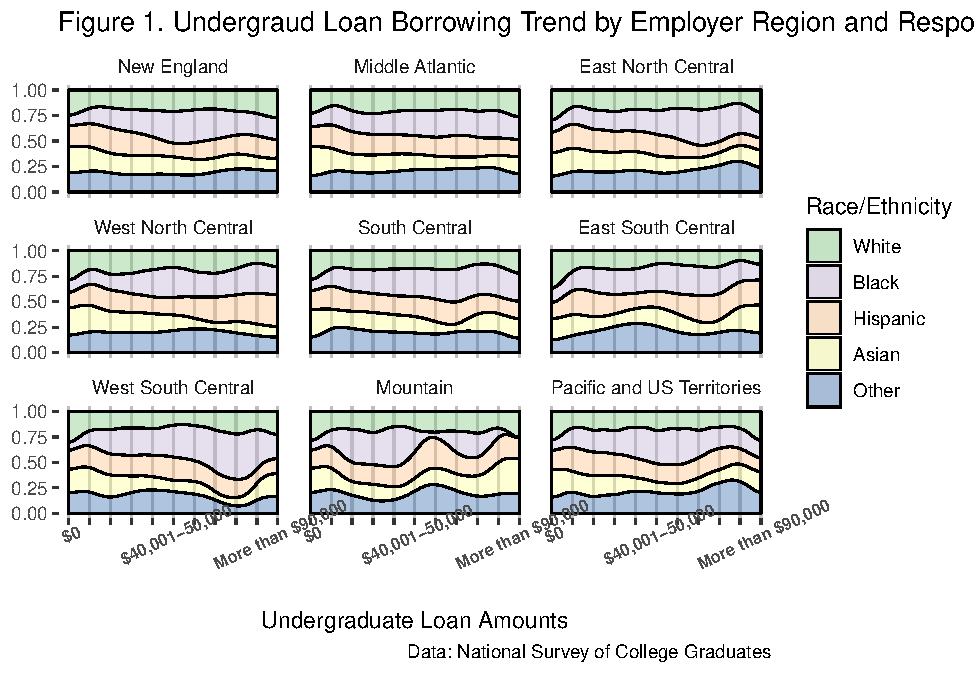
\includegraphics{Report_Draft_Test_files/figure-latex/unnamed-chunk-2-1.pdf}
In Figure 2, overall job satisfaction was generally lower for those with
higher loan amounts than those with any loans. However, there were few
instances where job satisfaction was highest for the higher loan amount
groups such as for those working in the Mountain, West South Central,
South Central, and West North Central regions. Figure 3 also revealed an
interesting pattern of the highest loan amount group (\$90,000 or more)
having almost as high satisfaction levels as those with zero loans for
Hispanics, Asians, and other race groups. This trend of higher
satisfaction levels for those with very high loan amounts suggests a
quadratic relationship where the satisfaction level drops when you go
from no loans to some loans and goes up again after certain amounts of
loan. Another interesting observation we made was that variation in
satisfaction levels are much wider in certain groups. For instance, when
we look at by race, the variation in the average satisfaction level by
loan amounts is very small for white and Asian respondents with data
range of about 3 percentage points, whereas black respondents had a
range of about 9 percentage points and other race respondents with 10
percentage points. This indicates that loan amounts many affect job
satisfaction differently by race or factors correlated with race.
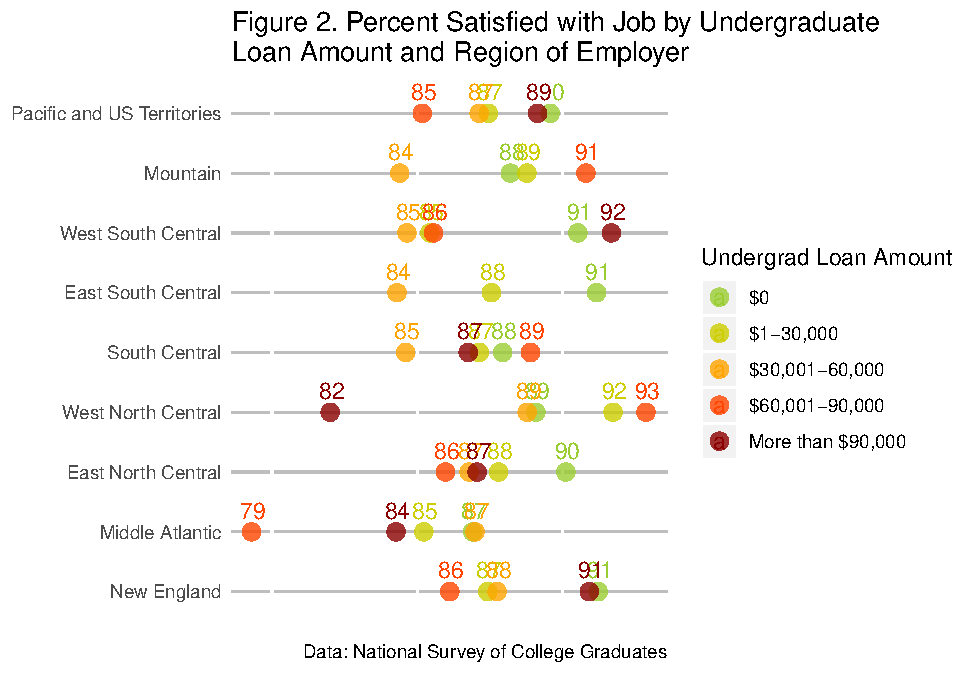
\includegraphics{Report_Draft_Test_files/figure-latex/unnamed-chunk-3-1.pdf}

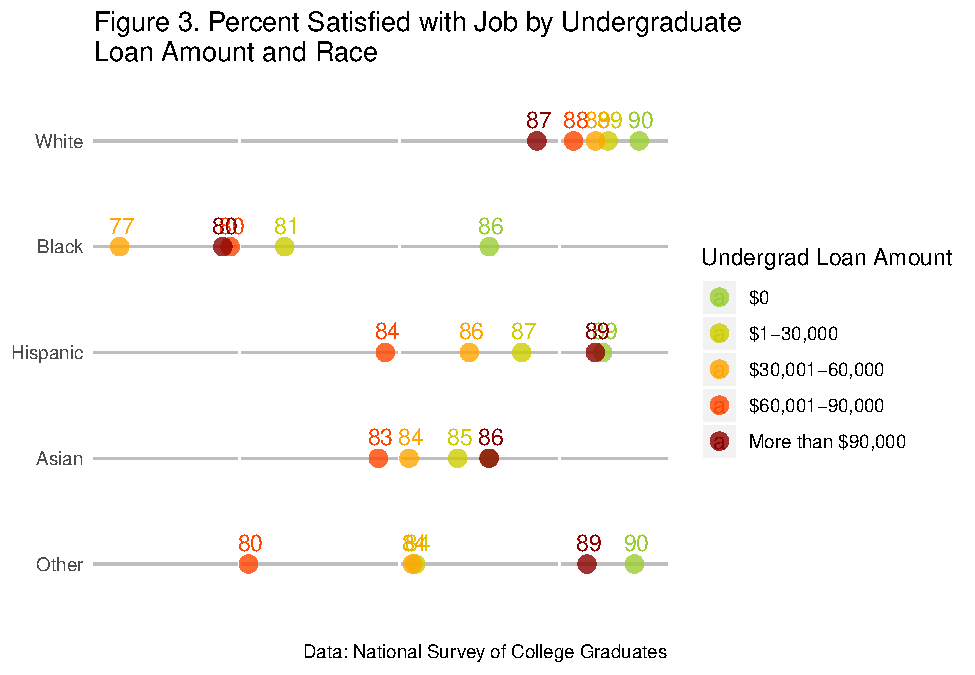
\includegraphics{Report_Draft_Test_files/figure-latex/unnamed-chunk-4-1.pdf}
Figure 4 through 8 are showing the changes in satisfaction levels over
loan amounts by various characteristics of the respondents. Overall,
these visualizations did not show a singular relationship between
undergraduate loan amounts and satisfaction levels. Some analysis groups
showed almost no change in satisfaction levels with increasing loan
amounts, whereas others showed random spikes or dips in the satisfaction
levels. However, a quadratic relationship that was also noted in Figure
2 was also observed in several of the analysis groups, suggesting that a
non-linear relationship between loan amounts and satisfaction levels.

Satisfactions in the job, security, and responsibility were the highest
among all job satisfaction categories and they aligned with each other
in terms of satisfaction levels and degree of change. Few of the plots,
such as the plot for New England region, university jobs, and federal
and state jobs, had one of the three satisfaction categories diverge off
from each other. Regardless of these few exceptions, these figures seem
to suggest that there is a high correlation among overall, security, and
responsibility at the job.

In some cases, we had satisfaction categories with generally lower
levels to show higher satisfaction level than the overall satisfaction
category as in the case of federal and state government jobs. In this
group, the satisfaction levels for job benefits and security were
noticeably higher than that of the overall satisfaction for all
undergraduate loan amounts. That is an expected result considering that
government jobs are well known for their job security and benefits.

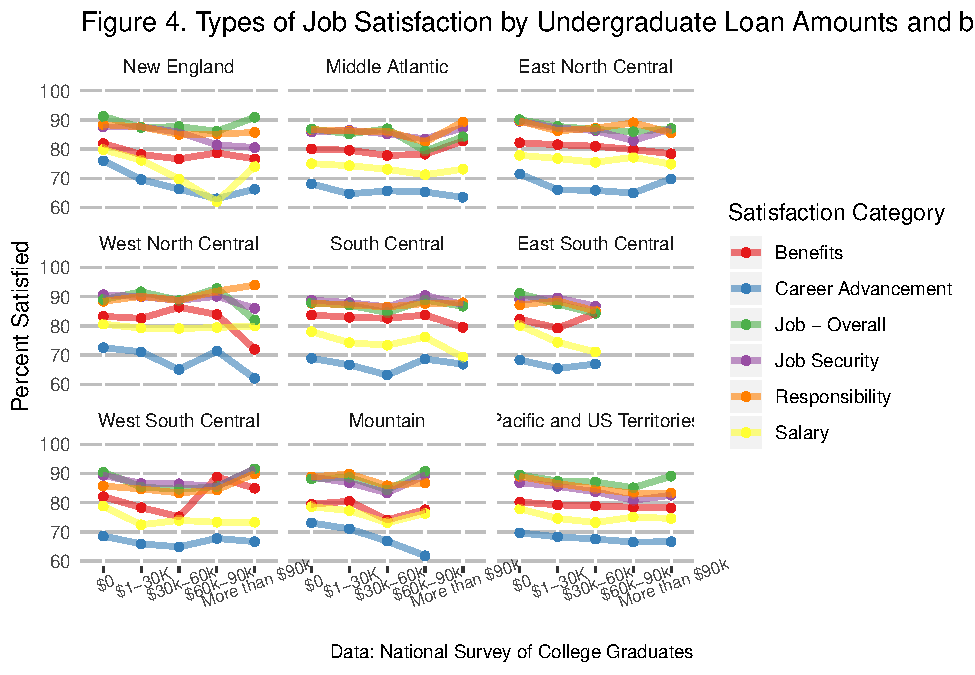
\includegraphics{Report_Draft_Test_files/figure-latex/unnamed-chunk-5-1.pdf}

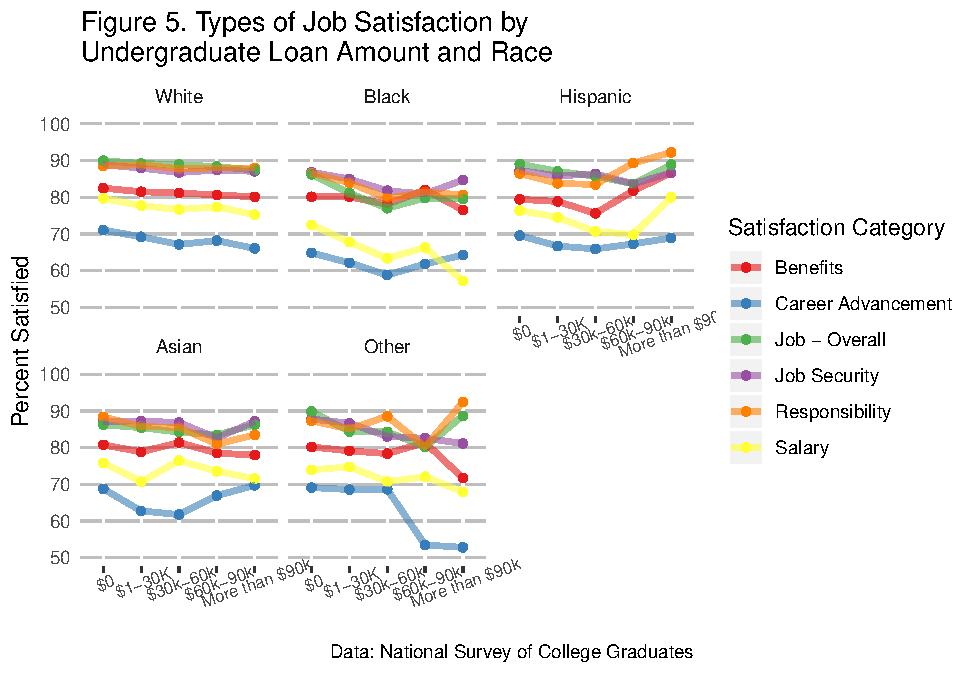
\includegraphics{Report_Draft_Test_files/figure-latex/unnamed-chunk-6-1.pdf}

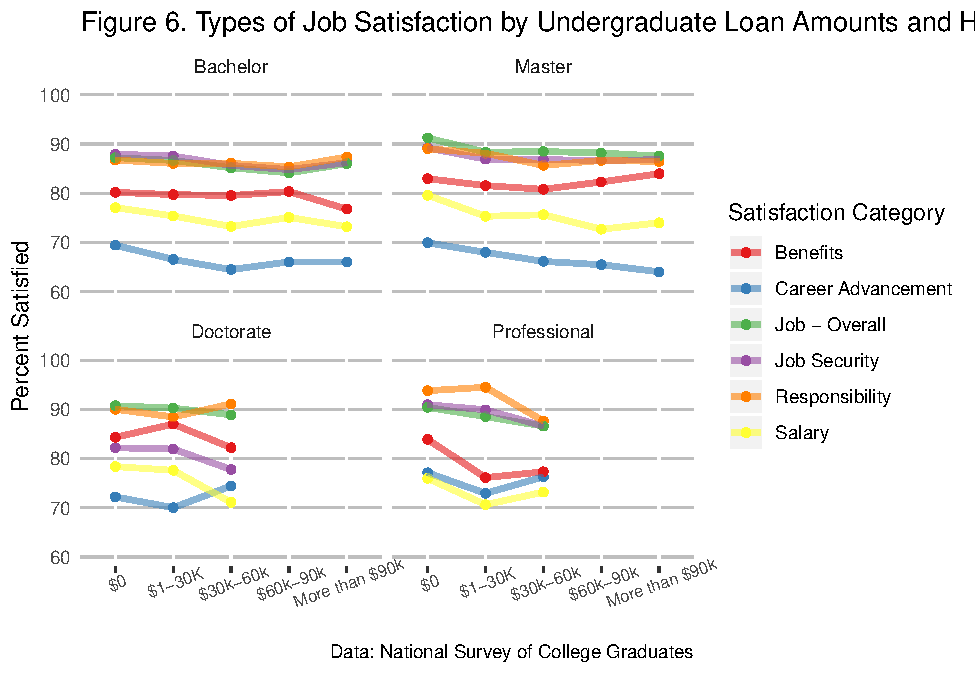
\includegraphics{Report_Draft_Test_files/figure-latex/unnamed-chunk-7-1.pdf}

\begin{verbatim}
## Warning: Removed 4 rows containing missing values (geom_point).
\end{verbatim}

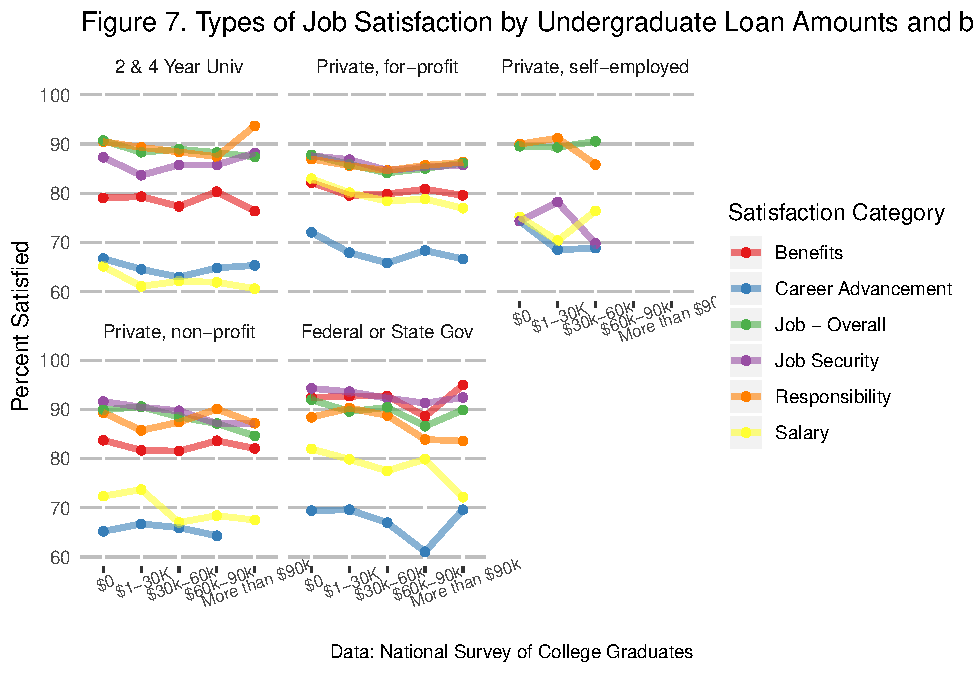
\includegraphics{Report_Draft_Test_files/figure-latex/unnamed-chunk-8-1.pdf}
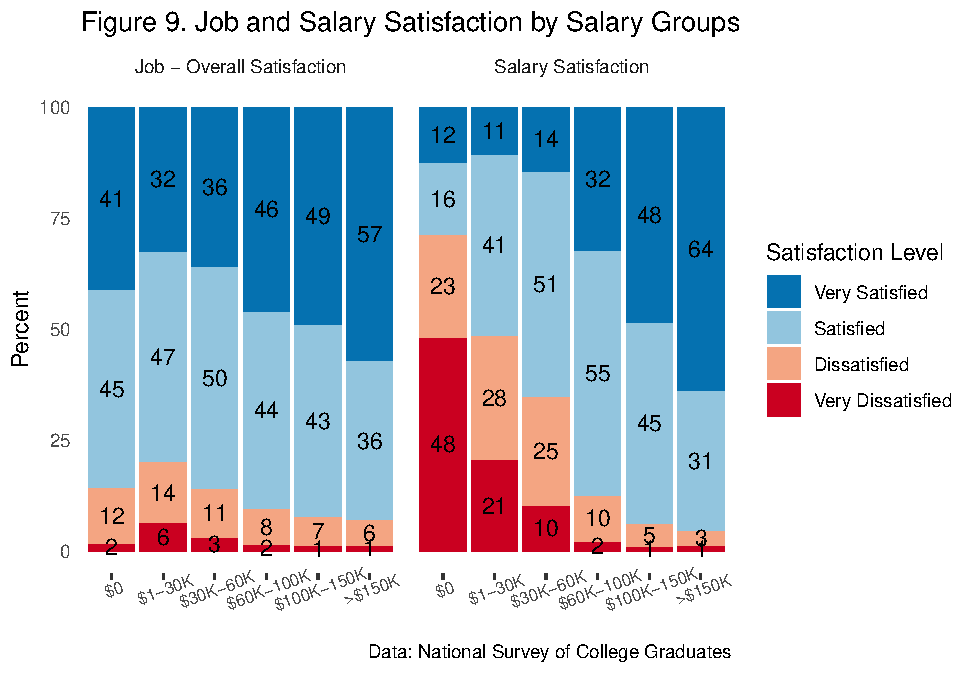
\includegraphics{Report_Draft_Test_files/figure-latex/unnamed-chunk-9-1.pdf}
In figures 9and 10, we created bar charts to show the distribution of
the responses for job satisfaction questionnaire over salary and age
groups. The percent of satisfied and very satisfied responses increased
with increasing salary amounts and age. However, the changes were very
small and, therefore, difficult to be claimed as meaningful. Through
this visual analysis method, we found few patterns that suggested
quadratic relationships between our dependent and independent variables.
However, the satisfaction levels were generally very high (around 85\%)
and had small variations in them, which meant that there was little room
for meaningful variations to be observed. And because this analysis is
limited to three variables at a time, these relationships cannot be
interpreted as casual or definitive as there could be omitted variable
bias that is affecting the relationships observed.

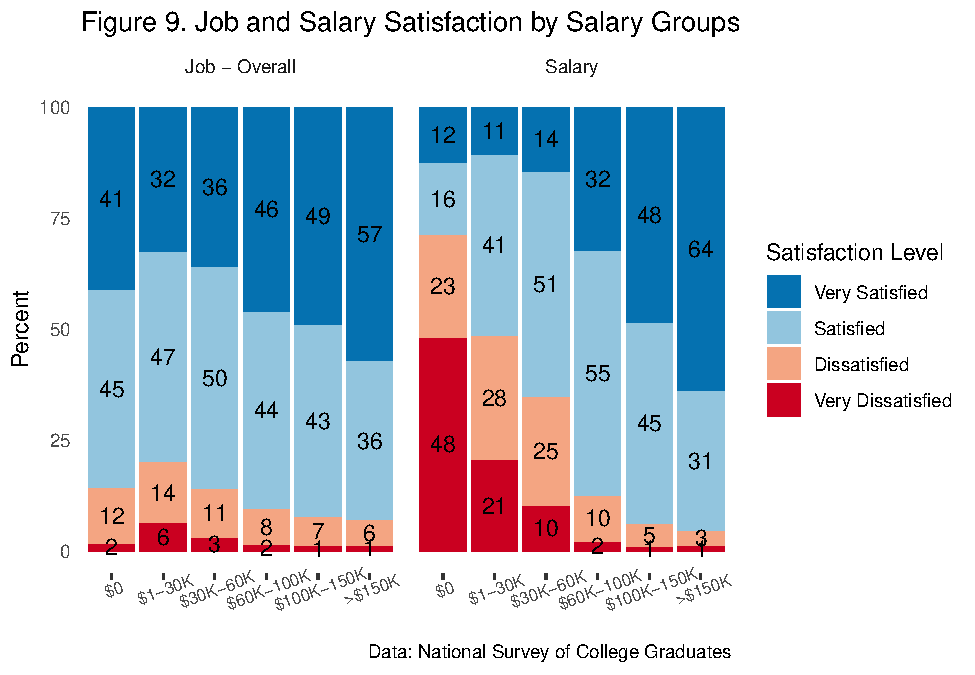
\includegraphics{Report_Draft_Test_files/figure-latex/unnamed-chunk-10-1.pdf}

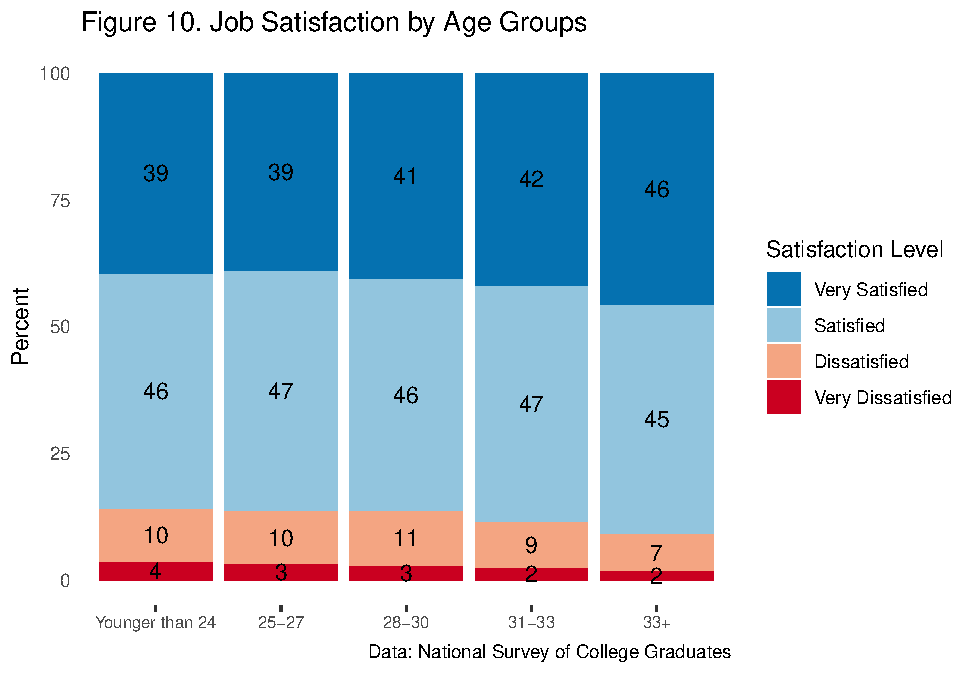
\includegraphics{Report_Draft_Test_files/figure-latex/unnamed-chunk-11-1.pdf}


\end{document}
